\capitulo{3}{Conceptos teóricos}

Antes de empezar con el desarrollo del proyecto, es necesario explicar una serie de conceptos teóricos.

\section{Sonido}

El sonido es una vibración mecánica que se propaga a través de un medio elástico, como el aire, el agua o cualquier otro material. Estas vibraciones generan diferencias de presión en el medio, que son captadas por nuestros oídos y percibidas como sonido.

Matemáticamente, el sonido se puede representar mediante una función matemática $g(t)$, donde $t$ representa el tiempo. Esta función describe cómo varía la presión o desplazamiento de partículas en el medio a medida que pasa el tiempo.

\subsection{Representación Matemática del Sonido}

La representación matemática más común del sonido es la onda sinusoidal. Una onda sinusoidal se puede describir mediante la siguiente ecuación \cite{Benson_2007}:

\begin{equation}
g(t) = A \sin(2\pi ft + \phi)
\end{equation}

Donde:
\begin{itemize}
\item $A$ es la amplitud de la onda, que representa la máxima desviación de la onda desde su posición de equilibrio.
\item $f$ es la frecuencia de la onda, que determina la cantidad de ciclos completos que la onda realiza en un segundo.
\item $t$ es el tiempo.
\item $\phi$ es la fase inicial de la onda, que determina el desplazamiento horizontal de la onda en el tiempo.
\end{itemize}

\section{Reconocimiento musical}

El reconocimiento musical es un área que se centra en el análisis de las características del audio, para así, extraer información relevante. Por ejemplo la identificación de canciones, géneros musicales, o artistas.

\subsection{Características del Sonido}

El reconocimiento musical se basa en el análisis de diversas características del sonido. Algunas de las características más comunes son:

\begin{itemize}
\item \textbf{Ritmo}: El ritmo es una de las propiedades fundamentales de la música y se refiere a la organización temporal de los eventos sonoros. Su complejidad abarca desde un ritmo repetitivo a un ritmo con notas y silencios complejos.
El ritmo se puede analizar en términos de su complejidad, regularidad, velocidad y otros aspectos. En algunos géneros de música, como el techno, el ritmo suele ser el aspecto más dominante.
La importancia del ritmo en el reconocimiento musical puede involucrar la detección del tempo y el análisis de los patrones rítmicos para obtener conclusiones. \cite{Crossley-Holland}

\item \textbf{Frecuencia}: La frecuencia musical es el número de vibraciones u oscilaciones por segundo en el sonido. 
La frecuencia de estas vibraciones se mide en ciclos por segundo, o hercios (Hz). Mientras mayor sea la frecuencia más agudo es el tono, y cuando menor más grave.
La frecuencia musical se puede utilizar para identificar notas específicas o para determinar la armonía.

\item \textbf{Timbre}: El timbre se refiere a las características tonales y armónicas que distinguen diferentes instrumentos y voces. 
Dos instrumentos musicales pueden reproducir la misma nota pero sonar de una manera completamente diferente debido a su timbre.
El análisis del timbre puede ayudar a reconocer estilos musicales debido a que permite identificar los diferentes instrumentos implicados en una canción.

\item \textbf{Estructura Musical}: La estructura musical se refiere a la organización global de una composición musical.
Estudiando la estructura musical se pueden distinguir las diferentes partes de una canción como el estribillo, versos o secciones instrumentales. De esta manera se pueden encontrar patrones repetitivos y que se ajusten a estilos musicales concretos. 
Por ejemplo una gran cantidad de la música pop \cite{Team} tiene una estructura definida como: 

\begin{center}
\hfill \textbf{Verso} - \hfill \textbf{Estribillo} - \hfill \textbf{Verso} - \hfill \textbf{Estribillo} - \hfill \textbf{Puente} - \hfill \textbf{Estribillo}
\end{center}

\end{itemize}

Este tipo de características o patrones comunes pueden ser utilizados por modelos de aprendizaje automático para aprender de los datos y extraer conclusiones.

\subsection{Aplicaciones del Reconocimiento Musical}
El reconocimiento musical tiene diversas aplicaciones prácticas y de gran uso en la actualidad, algunas de las cuales son:

\begin{itemize}
\item \textbf{Recomendación de música}: Los algoritmos de reconocimiento musical se utilizan para recomendar música a los usuarios en función de sus preferencias y patrones de escucha. 
Estos sistemas analizan las características de las canciones más escuchadas por el usuario y crean un modelo de recomendación basado en sus gustos.

\item \textbf{Clasificación de géneros musicales}: El reconocimiento musical se utiliza para clasificar automáticamente las canciones en diferentes géneros musicales, lo que facilita la organización y la búsqueda de música en grandes bibliotecas digitales.
\end{itemize}

\section{Ejemplo teórico de extracción de características musicales}

\subsection{Espectrograma}
Un espectrograma es una representación visual del espectro de frecuencia de una señal de audio en función del tiempo. 
Proporciona información detallada sobre cómo se distribuye la energía del sonido en diferentes frecuencias a lo largo del tiempo.

A continuación se explica el proceso para obtener un espectrograma de una canción.

\begin{itemize}
\tightlist
\item \textbf{Preprocesamiento de la señal de audio}: La señal de audio de la canción se divide en segmentos. De esta manera es posible analizar la variación espectral en diferentes puntos de la señal a lo largo del tiempo.

\item \textbf{Transformada de Fourier de tiempo corto (STFT)}: Cada segmento de la señal se somete a una transformada de Fourier de tiempo corto (STFT). La STFT divide la señal en múltiples segmentos de tiempo y calcula la suma de diferentes frecuencias en cada segmento. 
Esto se logra mediante la aplicación de una ventana temporal a cada segmento y luego calculando la transformada de Fourier de cada ventana.

\item \textbf{Cálculo de la magnitud del espectro}: La STFT proporciona diversa información sobre las fases y amplitudes de las frecuencias en cada segmento de tiempo. Sin embargo, para construir un espectrograma, generalmente se toma la magnitud del espectro (amplitud absoluta de las frecuencias).

\item \textbf{Representación visual}: La magnitud del espectro se representa visualmente en un gráfico 2D, donde el eje horizontal representa el tiempo y el eje vertical representa las frecuencias. La intensidad del color o brillo en cada punto del gráfico indica la energía o amplitud de la frecuencia correspondiente.
\end{itemize}

Los espectrogramas tienen una gran utilidad no solo en el estudio de la música. Por ejemplo, se pueden utilizar para visualizar las señales de un radar y detectar objetos o en lingüística estudiando los patrones de frecuencia de los sonidos del habla y así estudiar los diferentes fonemas o acentos.

\imagen{example_spectrogram}{Espectrograma de una pista de audio.}{1.0}

\newpage

\subsection{Coeficientes Cepstrales de Frecuencias de Mel (MFCC)}
Los coeficientes cepstrales de frecuencias de Mel (MFCC) son características ampliamente utilizadas en el procesamiento de señales de audio y el reconocimiento de voz. 
Estos coeficientes representan las características espectrales de una señal de audio en función de la escala de Mel, que es una escala perceptual de frecuencia basada en la respuesta del oído humano. \cite{SAHIDULLAH2012543} \cite{Deruty_2022}

A continuación se explica el proceso para obtener los coeficientes MFCC de una pista de audio.

\begin{enumerate}
\tightlist
\item \textbf{Preénfasis}: La señal de audio se normaliza con un filtro de preénfasis, que resalta las altas frecuencias y compensa la atenuación de las más bajas. Esto ayuda a mejorar la relación señal-ruido y realzar las características relevantes en el espectro.

\item \textbf{División en tramas}: La señal preénfasis se divide en tramas o segmentos cortos y superpuestos en el tiempo. Esto se hace para capturar la variación espectral en diferentes puntos de la señal a lo largo del tiempo.

\item \textbf{Cálculo de la Transformada de Fourier de tiempo corto (STFT)}: A cada trama de la señal se le aplica la Transformada de Fourier de tiempo corto (STFT), que calcula la contribución de diferentes frecuencias en cada trama. La STFT proporciona diversa información sobre las fases y amplitudes de las frecuencias en cada segmento de tiempo.

\item \textbf{Banco de filtros de Mel}: Se aplica un banco de filtros de Mel, que consiste en una serie de filtros triangularmente espaciados en la escala de Mel. Estos filtros se utilizan para representar el espectro en términos de bandas de frecuencia de Mel.

\item \textbf{Logaritmo de la energía}: Se calcula el logaritmo de la energía después de aplicar el banco de filtros de Mel. Esto se hace para tener en cuenta la respuesta no lineal del oído humano a las frecuencias.

\item \textbf{Transformada de Coseno Discreta}: Se aplica la Transformada de Coseno Discreta (DCT) a los valores obtenidos anteriormente.

\item \textbf{Extracción de los coeficientes MFCC}: Finalmente, se seleccionan los coeficientes cepstrales más significativos para representar la información espectral de la señal de audio. Estos coeficientes son los utilizados como características para aplicaciones de procesamiento y reconocimiento de audio.
\end{enumerate}

Los coeficientes MFCC son ampliamente utilizados en aplicaciones como: 

\begin{itemize}
\tightlist
\item Reconocimiento de voz: Como los MFCC son una forma de reducir la complejidad de la voz a estructuras más simples y fácilmente procesables, son utilizados para el reconocimiento de voz. Por ejemplo asistentes de audio como Siri o Alexa utilizan (junto a otros sistemas) MFCCs. \cite{Kiran_2021}
\item Identificación de hablantes: Los MFCC se pueden utilizar para identificar voces de diferentes hablantes, debido a que cada persona tiene una forma característica de hablar. \cite{Kiran_2021} \cite{Nakagawa_Wang}
\item Clasificación de audio: Se pueden utilizar para identificar diferentes sonidos o instrumentos musicales en una pista de audio y de esta manera obtener información relevante que permita realizar una clasificación. \cite{Wu}
\end{itemize}

\imagen{example_MFCC}{MFCC de una pista de audio.}{1.0}

\newpage

\section{Inteligencia Artificial}

La inteligencia artificial (IA) es la capacidad de un sistema informático de imitar funciones cognitivas humanas, como el aprendizaje y la solución de problemas

Los sistemas de inteligencia artificial pueden analizar grandes cantidades de datos, reconocer patrones y tomar decisiones basadas en esa información. Pueden aprender de la experiencia y mejorar su rendimiento con el tiempo. 

Hay diferentes enfoques en la IA, incluyendo el aprendizaje automático (\textit{machine learning}), el procesamiento del lenguaje natural (\textit{natural language processing}), la visión por computador (\textit{computer vision}) y la robótica, entre otros.

La IA se utiliza en una amplia variedad de aplicaciones cómo en sistemas de recomendación, análisis de datos o diagnósticos médicos por ejemplo.

\subsection{Aprendizaje automático (Machine Learning)}
El aprendizaje automático (\textit{machine learning}) es un subcampo de la inteligencia artificial que se centra en el desarrollo de algoritmos y modelos que permiten a los sistemas aprender y extraer información a partir de datos, sin ser explícitamente programados para ello.
Existen diversos tipos de aprendizaje automático:

\begin{itemize}
\item \textbf{Aprendizaje supervisado}: Se proporciona como entrada a los algoritmos un conjunto de datos de entrenamiento etiquetados. El modelo aprende a realizar predicciones o tomar decisiones basadas en estos ejemplos etiquetados. El aprendizaje supervisado se utiliza en tareas de clasificación o regresión.

\item \textbf{Aprendizaje no supervisado}: Los algoritmos trabajan con conjuntos de datos no etiquetados, es decir, sin clase conocida. El objetivo es encontrar patrones u estructuras ocultas en los datos. El aprendizaje no supervisado se utiliza en tareas como el agrupamiento (\textit{clustering}) o la detección de valores atípicos (\emph{outliers}).

\item \textbf{Aprendizaje por refuerzo}: En este tipo de aprendizaje, un agente inteligente interactúa con su entorno y aprende a tomar decisiones según una serie de recompensas o penalizaciones. El objetivo es encontrar una política de actuación que maximize las recompensas recibidas. El aprendizaje por refuerzo es utilizado para entrenar agentes en videojuegos o en robótica. \cite{sutton2018reinforcement}

\item \textbf{Aprendizaje semi-supervisado}: En este tipo de aprendizaje el conjunto de datos no está completamente etiquetado, por lo tanto, el objetivo es maximizar el rendimiento del modelo a partir de los datos con clase conocida. \cite{chapelle2006ssl}
\end{itemize}

\section{Ejemplo de aprendizaje supervisado}

En este proyecto se va a utilizar un enfoque de IA utilizando aprendizaje supervisado, por lo que se va a detallar un ejemplo simple para entender su funcionamiento: \cite{DADA2019e01802}

\subsection{Objetivo}
Construir un modelo de aprendizaje automático para clasificar correos electrónicos como "<spam"> o "<no spam">.

\subsection{Conjunto de datos}
Conjunto de datos etiquetados que contiene 1000 correos electrónicos, donde cada correo tiene características como la frecuencia de ciertas palabras sospechosas de pertenecer a spam, la longitud del mensaje, la presencia de enlaces o imágenes, entre otros. \textbf{Además de incluir la clase a la que pertenece: "<Spam"> o "<No Spam">}.

\subsection{Preparación de los datos}
Se deben preparar los datos para el entrenamiento del modelo. 
Una opción adecuada es representar cada correo electrónico como un vector de características.

\begin{table}[ht]
\centering
\begin{tabular}{|c|c|c|c|c|}
\hline
\textbf{Correo} & \textbf{Palabras sospechosas} & \textbf{Longitud} & \textbf{Enlaces} & \textbf{Etiqueta} \\ \hline
1 & 1 & 120 & 0 & No spam \\
2 & 4 & 56 & 1 & Spam \\
3 & 1 & 352 & 2 & No spam \\
4 & 9 & 174 & 0 & Spam \\
\hline
\end{tabular}
\caption{Ejemplo de datos de entrenamiento en un problema de aprendizaje supervisado}
\end{table}

\subsection{Entrenamiento del modelo}
Una vez preparados los datos en un formato adecuado, estos son introducidos en un algoritmo de aprendizaje supervisado formando un modelo de aprendizaje automático. Por ejemplo Redes Neuronales Artificiales, Máquinas de Soporte Vectorial o Árboles de decisión.

\subsection{Predicción}
Una vez entrenado el modelo, se alimenta con datos externos y se realizan predicciones.

El algoritmo utilizado en el proyecto es más complejo y será explicado en detalle en las siguientes secciones.

\newpage

\section{Redes neuronales}
Para realizar el entrenamiento del modelo de aprendizaje automático se han utilizado redes neuronales. 
Las redes neuronales son una categoría de modelos de aprendizaje automático inspirados en la estructura biológica del cerebro humano. Se componen de nodos interconectados llamados neuronas, organizadas en capas, que trabajan juntas para procesar información y hacer predicciones.
La decisión de utilizar redes neuronales en lugar de otras técnicas de aprendizaje automático para el entrenamiento del modelo se basa en varios factores: \cite{9165253} \cite{Nandi_2021} 

\begin{itemize}
\tightlist

\item \textbf{Capacidad de modelado de características no lineales}: Partiendo sobre las bases asentadas a lo largo de este proyecto, las redes neuronales resultan ser especialmente útiles debido a la naturaleza compleja y no lineal de la música. Cada canción tiene numerosos componentes, como el ritmo, la melodía, la armonía, la instrumentación, el tempo, y el timbre, los cuales interactúan entre sí de maneras complejas para crear un género musical. Estas interacciones no son fácilmente modelables con técnicas lineales, y los géneros musicales no pueden ser claramente separados en base a solo una o dos características.

Las redes neuronales son capaces de entender estas relaciones y patrones no lineales al aprender representaciones internas de las canciones que capturan las características esenciales que definen cada género. Esto les permite realizar predicciones precisas del género musical, incluso en el caso de canciones que pueden fusionar elementos de varios géneros o que no se ajustan claramente a las definiciones de género establecidas.

\item \textbf{Capacidad para aprender automáticamente características}: En lugar de depender de la ingeniería manual de características, las redes neuronales son capaces de aprender representaciones útiles de los datos de entrada por sí mismas. Esto nos puede resultar particularmente beneficioso en tareas que requieren un alto nivel de comprensión de los datos, como el procesamiento de imágenes, texto o audio, como es nuestro caso. De este modo, estaremos utilizando una herramienta que en vez de depender de esta extracción manual de las características de las canciones, como los coeficientes de frecuencia mel, las características espectrales o el ritmo, es capaz de aprender automáticamente las representaciones más útiles a partir de los datos de audio brutos o preprocesados.

\item \textbf{Escalabilidad}: Las redes neuronales pueden manejar grandes volúmenes de datos y se benefician de la computación paralela, lo que las hace adecuadas para manejar las grandes cantidades de datos disponibles en muchos problemas modernos de aprendizaje automático. En el caso de la detección de géneros musicales, esta capacidad de las redes neuronales se vuelve imprescindible. Las bases de datos de canciones para entrenamiento y validación suelen ser enormes, comprendiendo miles o incluso millones de pistas, las cuales pueden ser eficientemente gestionadas a través de las redes neuronales, las cuales, partiendo de esta diversidad de ejemplos trabajarán para generar un modelo más robusto y preciso. 

\end{itemize}

Las redes neuronales se componen de los siguientes elementos: \cite{AGGARWAL_2023}
\begin{itemize}
\tightlist
\item \textbf{Neuronas}: entidad matemática inspirada en la neurona biológica. Es el componente básico de una red neuronal. 
\item \textbf{Capas}: las neuronas están organizadas por capas. Capa se refiere a un conjunto de neuronas que procesan información al mismo tiempo. Dependiendo de su posición en relación a los datos de entrada existen tres tipos de capas: capa de entrada, capas ocultas y capa de salida.
\item \textbf{Proceso de entrenamiento}: el proceso de entrenamiento de una red neuronal consiste en ajustar los pesos y sesgos de las neuronas de tal manera que el error entre las predicciones y los valores reales sea lo más pequeño posible. Existen diversos algoritmos para realizar este cálculo iterativo de los valores de cada neurona.
\end{itemize}

\subsection{Neuronas artificiales}
Una neurona artificial es una entidad matemática inspirada en una neurona biológica. Se utilizan para modelar la información que una red recibe, procesa y luego utiliza para tomar decisiones.
Al igual que las neuronas en el cerebro humano, una neurona artificial toma una serie de entradas y produce una salida. Cada entrada tiene un peso asociado, que ajusta el valor de esa entrada para la salida final. Los pesos y valores se ajustan durante el proceso de entrenamiento para mejorar el rendimiento de la red.

La neurona artificial suma las entradas ponderadas y luego aplica una función de activación para producir la salida. Las funciones de activación son necesarias para introducir no linealidad en la red, lo que permite que la red aprenda a partir de datos más complejos.

Hay varios tipos de neuronas diferenciadas por su función de activación. Algunos ejemplos podrían ser: \cite{Baheti} \cite{Gutpa_2022}

\textbf{Neurona umbral}: esta neurona aplica una función de umbral a las entradas. Si la suma ponderada de las entradas supera un cierto umbral, la neurona se activa.

La función de activación umbral se define de la siguiente manera:

\[
f(x) = \begin{cases}
    0, & \text{si } x < \text{umbral} \\
    1, & \text{si } x \geq \text{umbral}
\end{cases}
\]

Donde \text{umbral} es el valor de umbral que determina el punto de corte para la activación de la neurona.

\textbf{Neurona sigmoidal}: la neurona sigmoidal aplica una función sigmoide a las entradas

La función de activación sigmoidal se define de la siguiente manera:

\[
f(x) = \frac{1}{1 + e^{-x}}
\]

Donde $x$ es el valor de entrada de la neurona.

\textbf{Neurona ReLU \textit{(Rectified Linear Unit)}}: este tipo de neurona utiliza la función ReLU como su función de activación.
Este tipo de función de activación introduce no linealidad sin los problemas que pueden surgir con otras funciones de activación.

La función de activación ReLU se define de la siguiente manera:

\[
f(x) = \begin{cases}
    0, & \text{si } x < 0 \\
    x, & \text{si } x \geq 0
\end{cases}
\]

Donde $x$ es el valor de entrada de la neurona.

\textbf{Neurona softmax}: esta neurona se utiliza en la capa de salida para problemas de clasificación multiclase. La función Softmax toma un vector de entradas y produce un vector de salidas, cada una de las cuales está entre 0 y 1 y la suma total es 1. 
Cada salida puede interpretarse como la probabilidad de que la entrada pertenezca a una clase particular.

\[
f(x_i) = \frac{e^{x_i}}{\sum_{j=1}^{N} e^{x_j}}
\]

Donde $x_i$ es el valor de entrada de la neurona y $N$ es el número total de entradas.

\subsection{Capas}
Una red neuronal artificial está compuesta por un conjunto de capas neuronales interconectadas. \cite{AGGARWAL_2023} \cite{Ognjanovski_2020}
Cada capa consiste en un conjunto de neuronas las cuales reciben información de la capa anterior y envía su salida a las neuronas en la capa siguiente. Según su posición en la red neuronal las capas se pueden clasificar como:

\textbf{Capa de entrada}: es la primera capa de la red. Cada neurona en la capa de entrada corresponde a una característica en el conjunto de datos de entrada.

\textbf{Capas ocultas}: capas que se encuentran entre la capa de entrada y la capa de salida. Su número varía dependiendo de la profundidad de la red. 
En estas capas es donde se produce la mayor parte del cálculo de la red. Los pesos de las conexiones entre las neuronas en las capas ocultas se ajustan durante el entrenamiento.

\textbf{Capa de salida}: última capa de la red. Es la capa donde se devuelve la información. El número de neuronas en la capa de salida suele estar determinado por el tipo de problema que se está resolviendo. Por ejemplo, en un problema de clasificación binaria, solo se necesitaría una neurona de salida. En un problema de clasificación de varias clases, el número de neuronas de salida sería igual al número de clases.

\begin{figure}
\centering
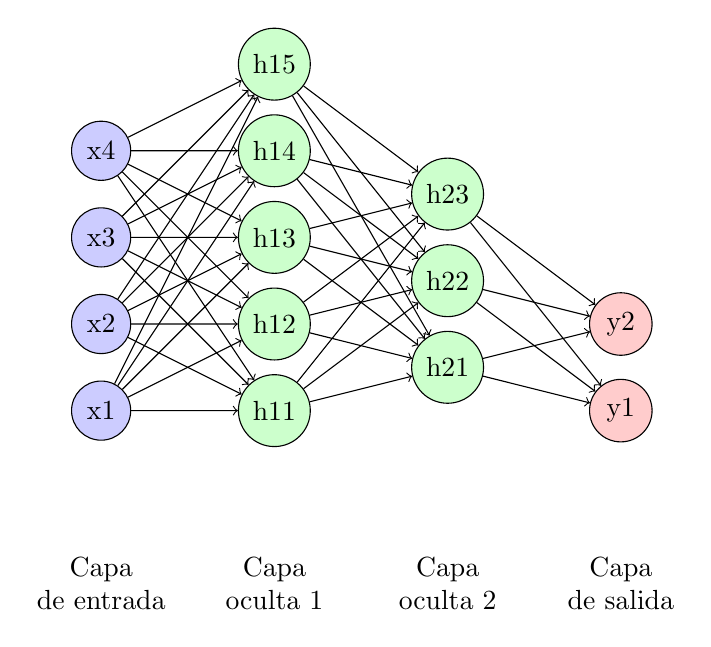
\begin{tikzpicture}[scale=1.1]
  % Capa de entrada
  \foreach \x in {1,...,4}
    \node[circle, draw=black, fill=blue!20] (input\x) at (0,\x) {x\x};

  % Capa oculta 1
  \foreach \x in {1,...,5}
    \node[circle, draw=black, fill=green!20] (hidden1\x) at (2,\x) {h1\x};

  % Capa oculta 2
  \foreach \x in {1,...,3}
    \node[circle, draw=black, fill=green!20] (hidden2\x) at (4,\x+0.5) {h2\x};

  % Capa de salida
  \foreach \x in {1,...,2}
    \node[circle, draw=black, fill=red!20] (output\x) at (6,\x) {y\x};

  % Conexiones
  \foreach \i in {1,...,4}
    \foreach \j in {1,...,5}
      \draw[->] (input\i) -- (hidden1\j);

  \foreach \i in {1,...,5}
    \foreach \j in {1,...,3}
      \draw[->] (hidden1\i) -- (hidden2\j);

  \foreach \i in {1,...,3}
    \foreach \j in {1,...,2}
      \draw[->] (hidden2\i) -- (output\j);

  % Etiquetas de capas
  \node[align=center] at (0,-1) {Capa\\de entrada};
  \node[align=center] at (2,-1) {Capa\\oculta 1};
  \node[align=center] at (4,-1) {Capa\\oculta 2};
  \node[align=center] at (6,-1) {Capa\\de salida};

\end{tikzpicture}
\caption{Red neuronal con dos capas ocultas \cite{Wikilibros}}
\end{figure}

\subsection{Tipos de capas}

Las redes neuronales se componen de varias capas cada una con su funcionalidad específica. A continuación se exploran algunos tipos comunes de capas. \cite{Rosebrock_2023}

\textbf{Capas densas o totalmente conectadas}: cada neurona está conectada a todas las neuronas en la capa anterior y a todas las neuronas en la capa siguiente.

\textbf{Capas convolucionales}: capas formadas por redes neuronales convolucionales. En lugar de conectarse a todas las neuronas de la capa anterior, una neurona en una capa convolucional está conectada a un pequeño subconjunto de las neuronas en la capa anterior.

\textbf{Capas recurrentes}: capas formadas por redes neuronales recurrentes. En una capa recurrente, las neuronas tienen conexiones de retroalimentación con ellas mismas a lo largo del tiempo.

\textbf{Capas de pooling}: capas utilizadas para reducir la dimensionalidad de los datos. Una capa de pooling toma un subconjunto de las entradas y produce una sola salida, que es una medida estadística resumida de sus entradas (por ejemplo, el máximo o el promedio).

\textbf{Capas de normalización}: capas utilizadas para normalizar las entradas a una red o las salidas de una capa anterior. La normalización ayuda con el proceso de entrenamiento de la red.

\section{Proceso de entrenamiento}
El entrenamiento de una red neuronal implica un proceso que, de forma iterativa, ajusta los pesos de cada una de las neuronas para minimizar la diferencia entre las salidas predichas y las salidas reales del conjunto de datos de entrenamiento. Este proceso se puede clasificar en varios pasos: \cite{Pramoditha_2022}

\textbf{Inicialización de pesos}: el primer paso en el entrenamiento es inicializar los pesos de las neuronas de la red. Normalmente se inicializan de manera aleatoria.

\textbf{Propagación hacia adelante}: la propagación hacia adelante es el proceso por el cual la red neuronal transmite la información desde la capa de entrada hasta la capa de salida mediante la información calculada en cada función de activación neuronal.

\textbf{Función de perdida}: proceso de medición de la calidad de las predicciones. La función de perdida (o función de coste) genera un valor indicando cuanta distancia existe entre las predicciones y las clases verdaderas. Existen distintos tipos de funciones de perdida, en el caso de este proyecto la función utilizada es \textit{Sparse Categorical Crossentropy}, esta función es utilizada en problemas de clasificación multiclase dónde las etiquetas son datos enteros como es el caso del proyecto. \cite{Koech_2022}
La función es la siguiente:

\begin{equation}
L = - \log(y_{\mathrm{pred}}[y_{\mathrm{true}}])
\end{equation}

Donde:
\begin{itemize}
\tightlist
\item $y_{\mathrm{pred}}$ son las probabilidades predichas para cada clase.
\item $y_{\mathrm{true}}$ es la etiqueta verdadera.
\end{itemize}

\textbf{Backpropagation}: proceso de ajuste de los pesos de la red neuronal en función al error calculado en la función de perdida. El objetivo es minimizar iterativamente la función de pérdida propagando los errores desde la capa de salida hacia las capas ocultas por medio de la regla de la cadena, de esta manera se puede descubrir que número de neuronas deben actualizar sus pesos. La técnica que hace posible este proceso es el Descenso del Gradiente. 

\textbf{Descenso del Gradiente}: algoritmo de optimización utilizado para minimizar la función de pérdida. Su funcionamiento consiste en ajustar los parámetros del modelo de forma iterativa en la dirección negativa del gradiente de la función de pérdida. Su función es la siguiente:

\begin{equation}
\theta_{j} = \theta_{j} - \alpha \frac{\partial}{\partial \theta_{j}} J(\theta)
\end{equation}

Donde:
\begin{itemize}
\tightlist
\item $\theta_{j}$ es el peso a actualizar.
\item $J(\theta)$ es la función de pérdida.
\item $\frac{\partial}{\partial \theta_{j}} J(\theta)$ es el gradiente de la función de pérdida con respecto al parámetro $\theta_{j}$.
\item $\alpha$ es la tasa de aprendizaje o \textit{learning rate}, este parámetro controla cuanto varía $\theta_{j}$ en cada iteración.
\end{itemize}

\textbf{Iteración}: todo este proceso se repite $N$ veces. Cada proceso completo de inicialización, propagación hacia adelante, función de coste y backpropagation se llama época (\textit{epoch}). Ejecutar demasiadas épocas puede provocar sobreajuste, por este motivo, se implementan criterios de parada. Estos criterios pueden ser un número fijo de épocas, la estabilización de la función de pérdida (cuando no mejora tras un cierto número de épocas), una tasa de error constante en un conjunto de prueba, o si la disminución en la función de pérdida es menor que una tolerancia establecida.

\section{Evaluación del modelo}
La evaluación de un modelo de red neuronal es el proceso donde se determina la efectividad del modelo. Este proceso debe realizarse durante y después del entrenamiento.

\textbf{Evaluación con el conjunto de prueba}: tras entrenar el modelo es imprescindible realizar una evaluación final con el conjunto de prueba. Esta evaluación da como resultado una evaluación más precisa de como se comportará el modelo con datos externos.

\subsection{Cálculo de métricas de rendimiento}
Existen diversas métricas de rendimiento que indican como de bueno es el entrenamiento del modelo. Algunas de las más usadas en problemas de clasificación son:

\textbf{Accuracy}: proporción de predicciones correctas que hace el modelo en relación con todas las predicciones que hace.
\begin{equation}
\text{Accuracy} = \frac{\text{TP} + \text{TN}}{\text{TP} + \text{FP} + \text{FN} + \text{TN}}
\end{equation}

\textbf{Recall}: recall es la proporción de instancias positivas que el modelo predice correctamente en relación con todas las instancias positivas reales.
\begin{equation}
\text{Recall} = \frac{\text{TP}}{\text{TP} + \text{FN}}
\end{equation}

\textbf{F1-Score}: media armónica de precisión y recall.
\begin{equation}
\text{F1-Score} = 2 \cdot \frac{\text{Precision} \cdot \text{Recall}}{\text{Precision} + \text{Recall}}
\end{equation}
